\chapter{Captura XADC y memoria FIFO}
\label{section:xadc_fifo}


Como se ha introducido anteriormente, en este capítulo se definirá el proceso de captura y conversión de una señal de entrada triangular y el posterior almacenamiento de la misma en una memoria FIFO. En la figura \ref{fig:xadc_fifo} se muestra el diseño de los bloques necesarios para esta fase y la definición de sus correspondientes puertos de entrada y salida.

\vspace{3mm}

    \begin{figure}[h]
    	\centering
    	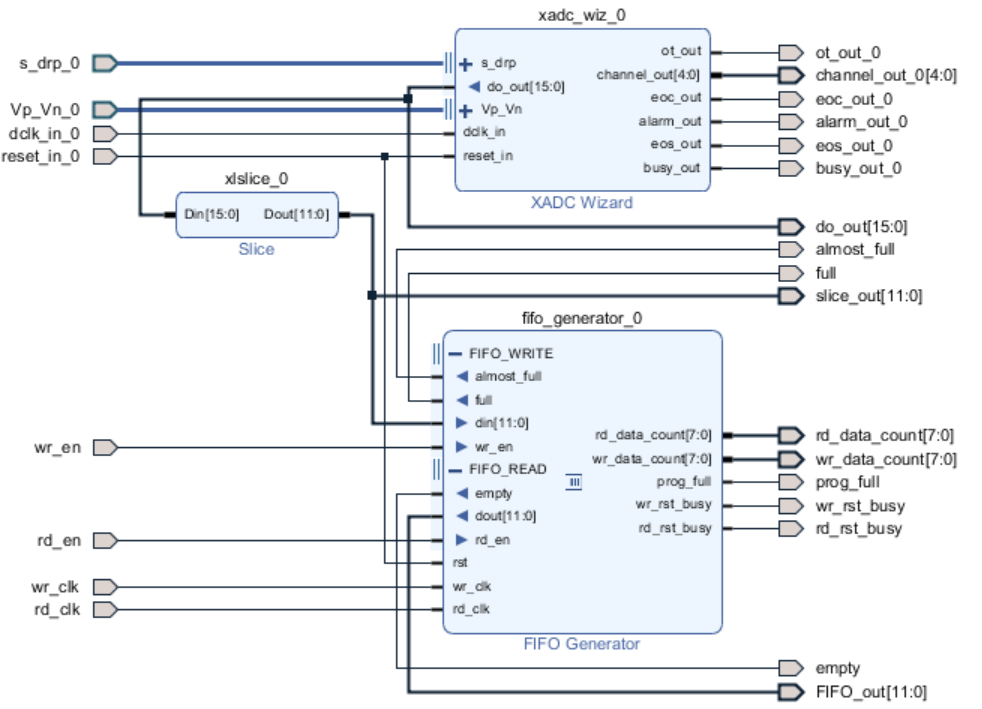
\includegraphics[width=1\textwidth]{img/diseno/xadc_fifo.PNG}
    	\caption{Diseño del bloque XADC+FIFO}
    	\label{fig:xadc_fifo}
    \end{figure}
    
\vspace{3mm}

\vspace{3mm}

    \begin{figure}[h]
    	\centering
    	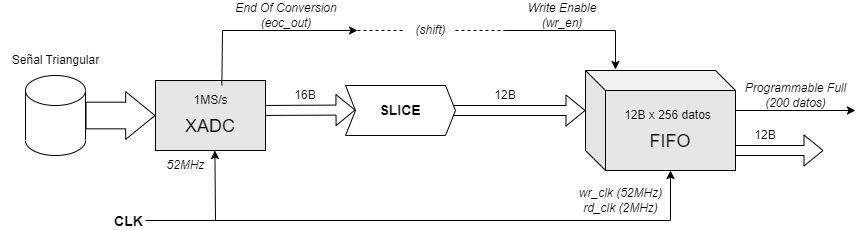
\includegraphics[width=1\textwidth]{img/diseno/xadc_fifo.drawio.PNG}
    	\caption{Diseño del bloque XADC+FIFO}
    	\label{fig:xadc_fifo}
    \end{figure}
    
\vspace{3mm}


\section{Obtención de los datos convertidos del ADC – simulación señal de entrada}



\section{Lógica de control de lectura/escritura de los datos de la FIFO. Comprobación del bloque FIFO}